%************************************************
\chapter{The Final Product}\label{ch:final}
%************************************************

Everything we have done and discussed in the previous chapters has been building up to this point. We can finally see the fruits of countless hours of work, planning, designing and developing the applications.

Let's take a walkthrough around all the implemented features, while also comparing and contrasting the differences and similarities between the iOS and Android versions.

The following screenshots have been taken directly from physical devices running the applications. For the iOS version, it is an iPhone 4 running iOS 7 and for the Android version a Samsung Galaxy Nexus running Android 4.4. The difference in screenshot size is due to the different screen size on each device. The iPhone has a 3.5 inch screen while the Nexus has a 4.65 inch screen.

Once you start the application you are greeted by a splash screen with a loading icon. This screen fades away once the application has finished fetching any new content. At this point the application communicates with the cloud service to check for new available Companies and pre-load their icons to the local storage.

\begin{figure}[H]
        \myfloatalign
        \subfloat[iOS]
        {
\includegraphics[width=.3\linewidth]{gfx/ios/splash}} \quad
        \subfloat[Android]
        {
\includegraphics[width=.3\linewidth]{gfx/and/splash}} \\
        \caption[Splash Screen]{Splash Screen}
\end{figure}
\newpage

The next thing you see is a list containing the latest Publications from the available companies.

\begin{figure}[H]
        \myfloatalign
        \subfloat[iOS]
        {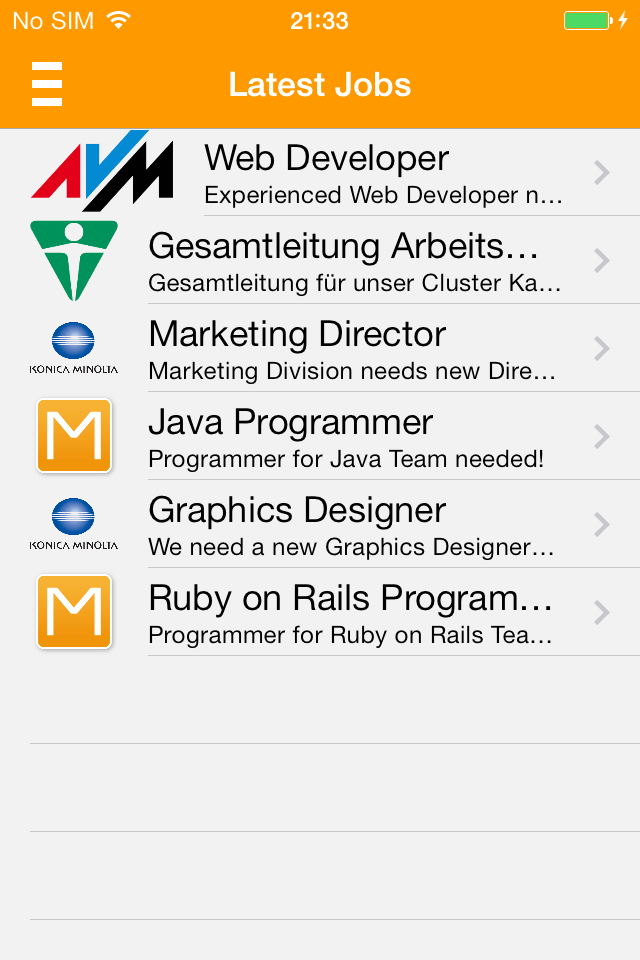
\includegraphics[width=.3\linewidth]{gfx/ios/main}} \quad
        \subfloat[Android]
        {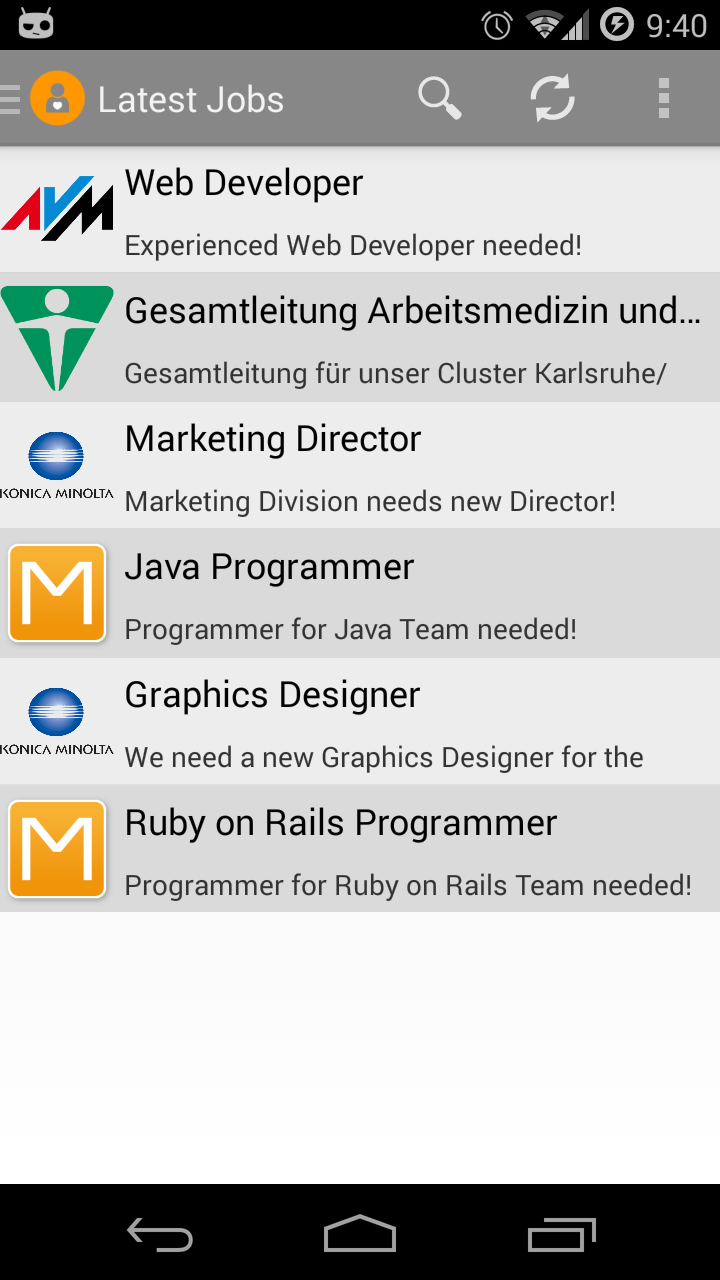
\includegraphics[width=.3\linewidth]{gfx/and/main}} \\
        \caption[Publications View]{Publications View}
\end{figure}

If you click on the menu icon, you'll see a second list slide form the left side of the screen. In here you'll find the entries for the navigation menu. You can go to the companies view, or return to the home view. You'll also notice a difference between iOS and Android. iOS has an extra entry on the menu for the search view, while Android can preform the search from the top bar.

\begin{figure}[H]
        \myfloatalign
        \subfloat[iOS]
        {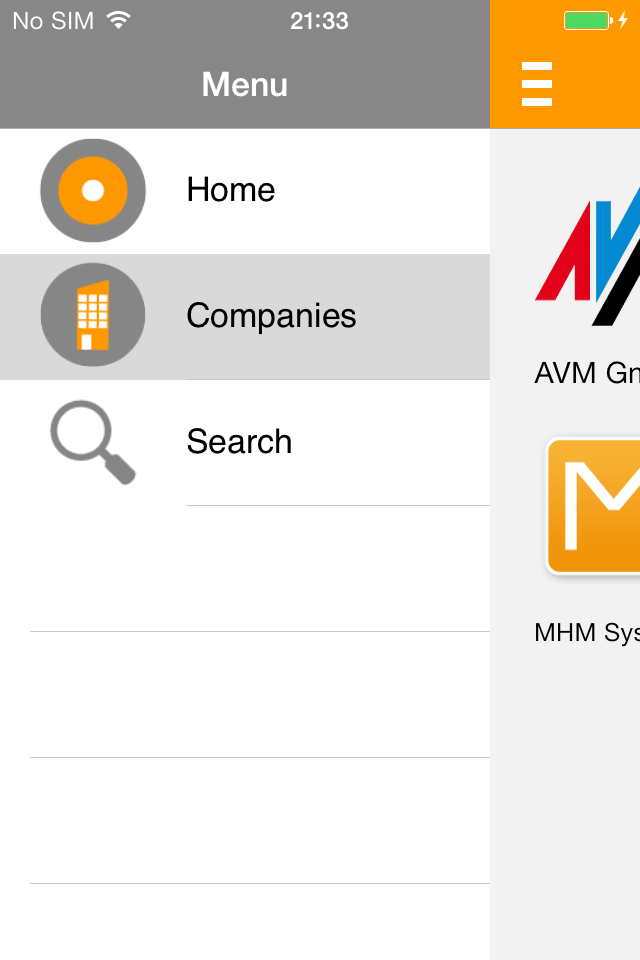
\includegraphics[width=.3\linewidth]{gfx/ios/menu}} \quad
        \subfloat[Android]
        {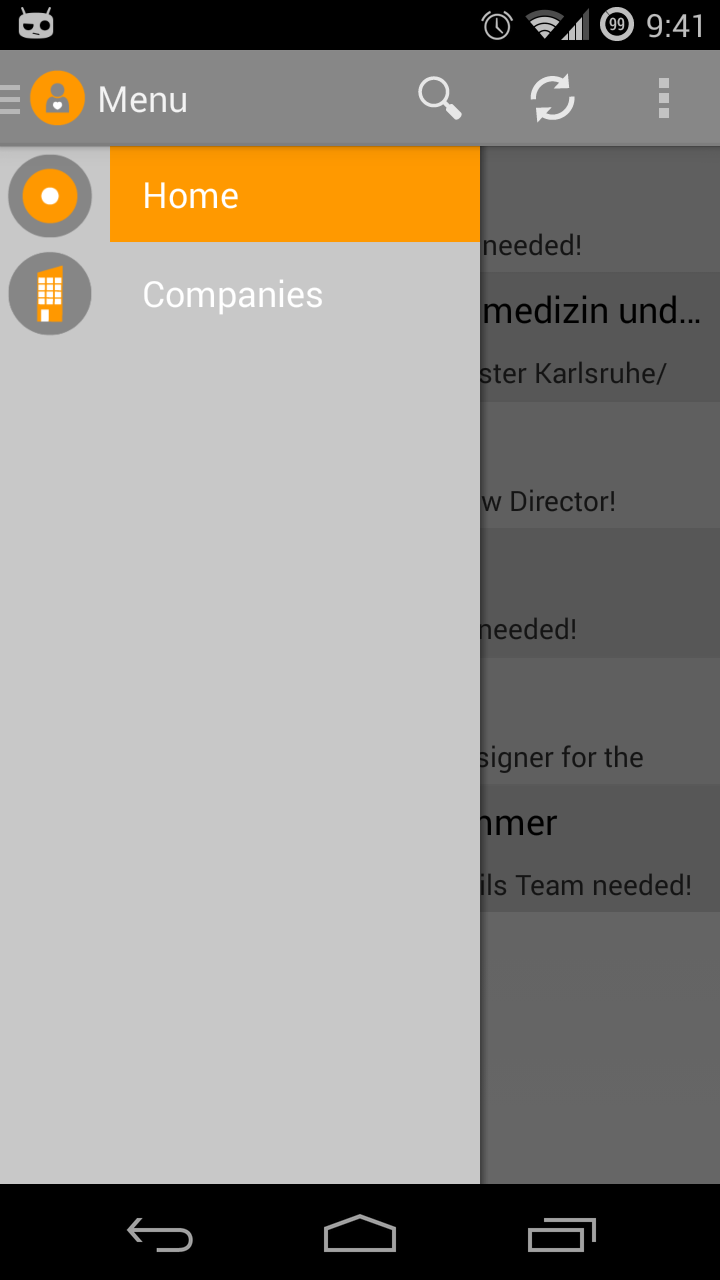
\includegraphics[width=.3\linewidth]{gfx/and/menu}} \\
        \caption[Menu]{Menu}
\end{figure}
\newpage

From there we can go the the companies view and see a grid with the available companies.

\begin{figure}[H]
        \myfloatalign
        \subfloat[iOS]
        {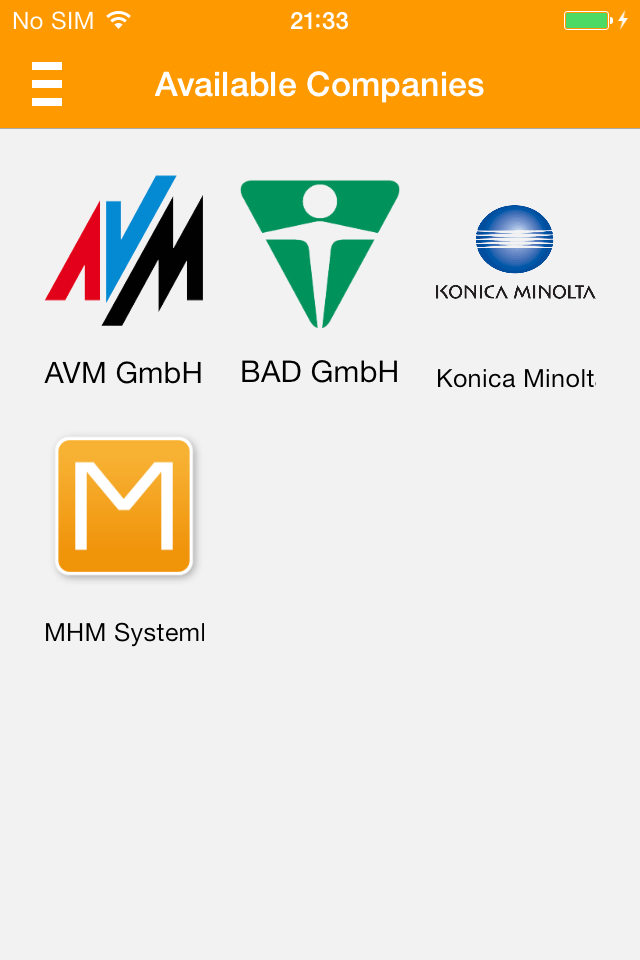
\includegraphics[width=.3\linewidth]{gfx/ios/companies}} \quad
        \subfloat[Android]
        {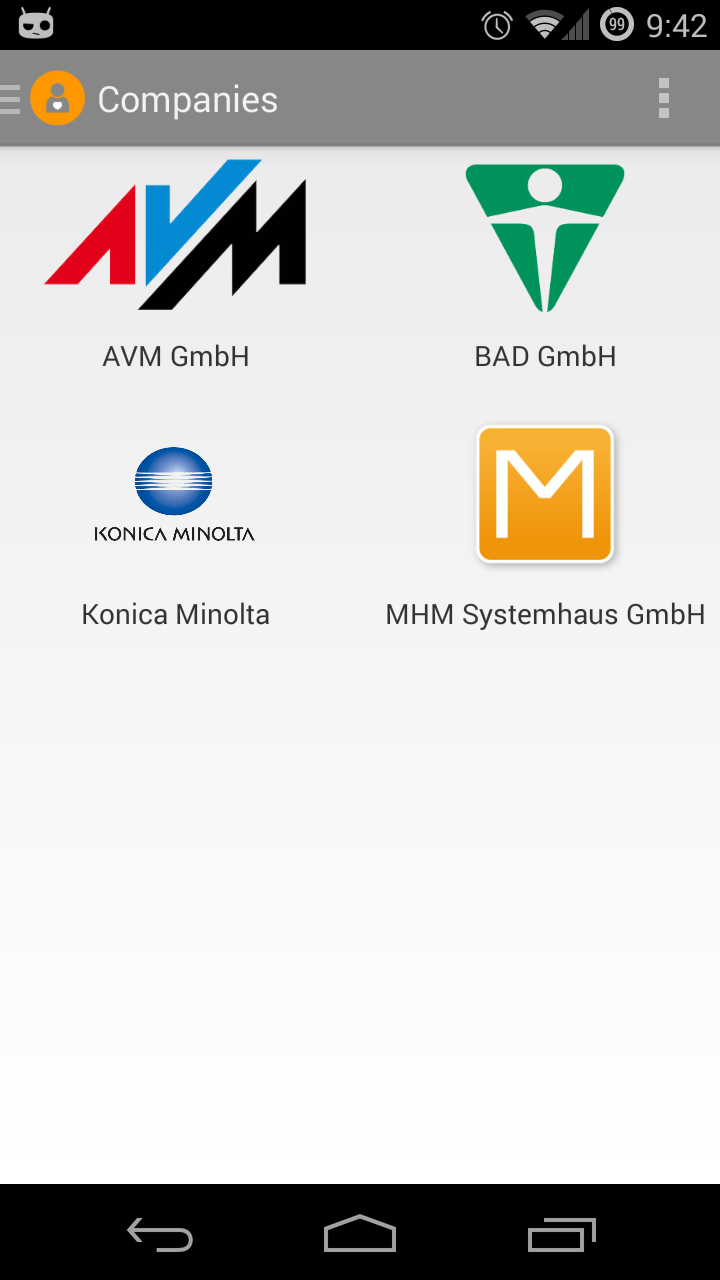
\includegraphics[width=.3\linewidth]{gfx/and/companies}} \\
        \caption[Companies View]{Companies View}
\end{figure}

Let's continue moving forward and click on a company. We will be greeted by a very similar view as the home view, but with filtered publications.

\begin{figure}[H]
        \myfloatalign
        \subfloat[iOS]
        {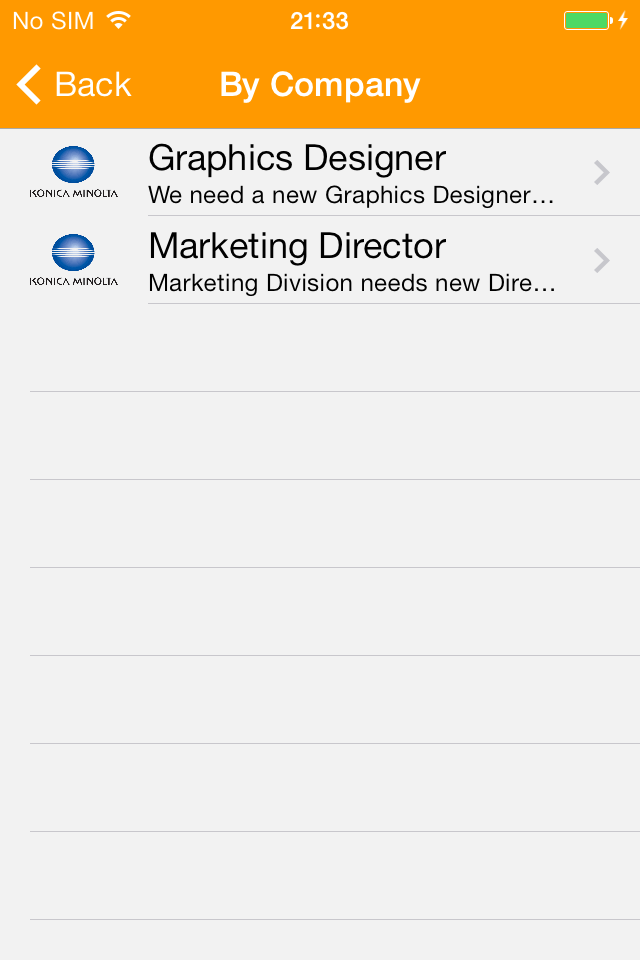
\includegraphics[width=.3\linewidth]{gfx/ios/filtered}} \quad
        \subfloat[Android]
        {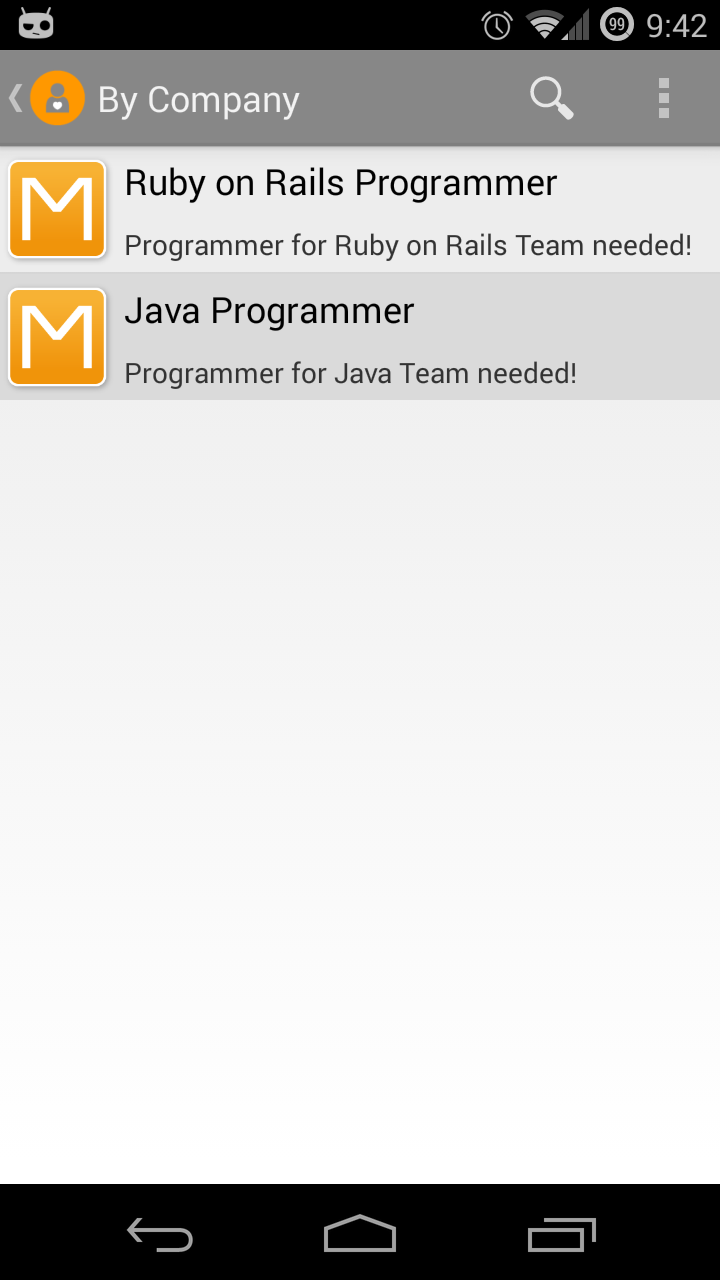
\includegraphics[width=.3\linewidth]{gfx/and/filtered}} \\
        \caption[Filtered View]{Filtered View}
\end{figure}

Let's now click on a Publication to see more details about it. A new view appears. This new view disables the menu icon and replaces it with a back button for navigation.

\begin{figure}[H]
        \myfloatalign
        \subfloat[iOS]
        {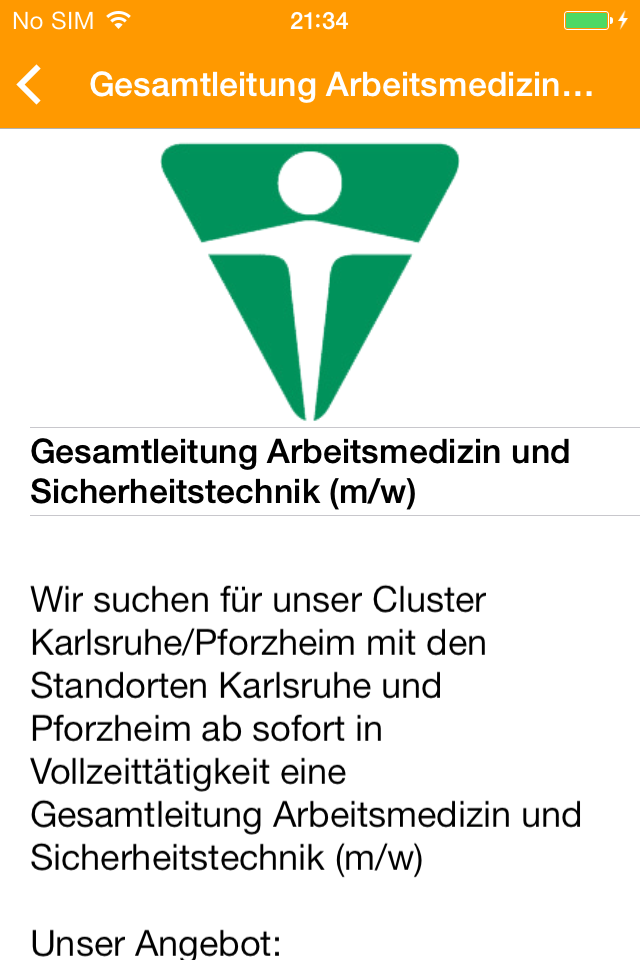
\includegraphics[width=.3\linewidth]{gfx/ios/job}} \quad
        \subfloat[Android]
        {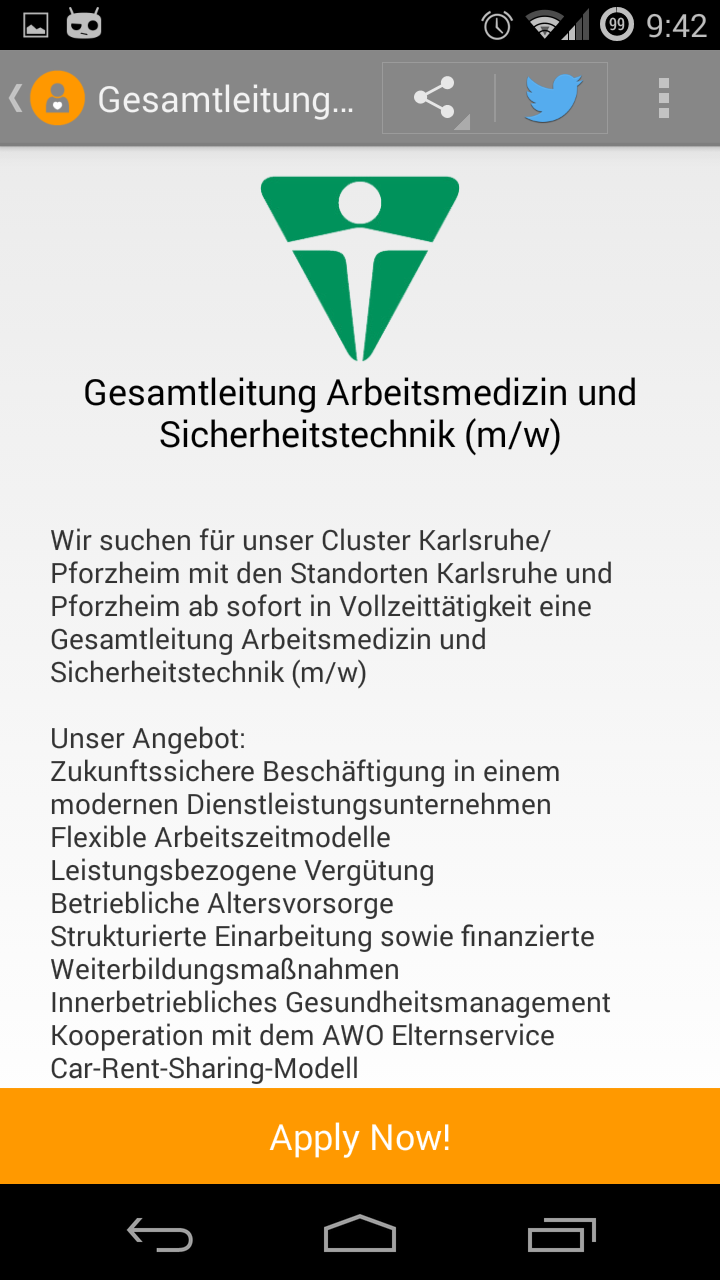
\includegraphics[width=.3\linewidth]{gfx/and/job}} \\
        \caption[Filtered View]{Filtered View}
\end{figure}

Inside this view you'll also see an "Apply Now!" button (iOS users need to scroll to the bottom). If you click this button you will be taken to a web view, that let's you directly apply to this vacancy via the responsive web interface of the \textit{MHM eRecruiting Application}.

\begin{figure}[H]
        \myfloatalign
        \subfloat[iOS]
        {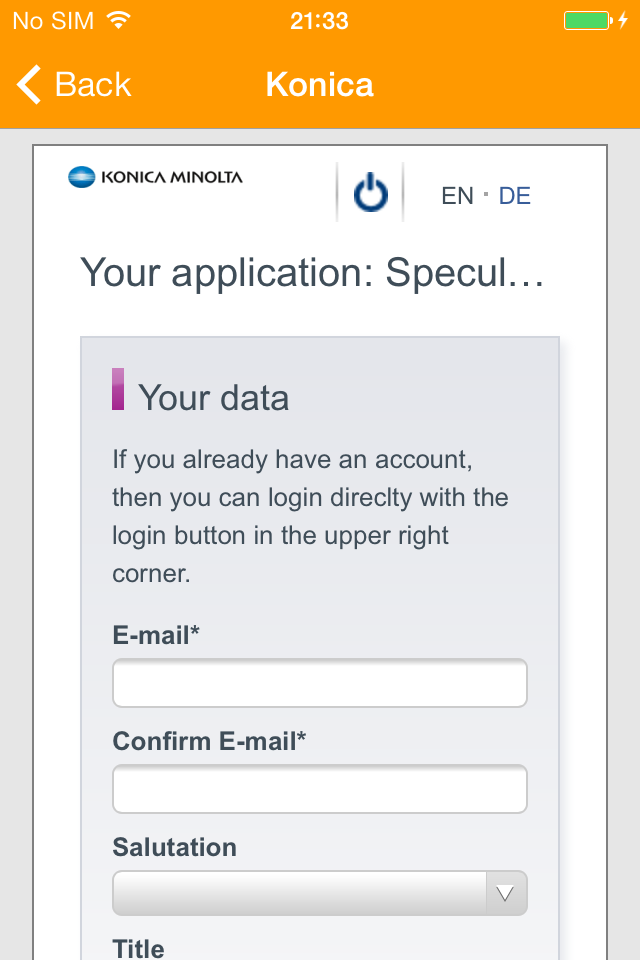
\includegraphics[width=.3\linewidth]{gfx/ios/web}} \quad
        \subfloat[Android]
        {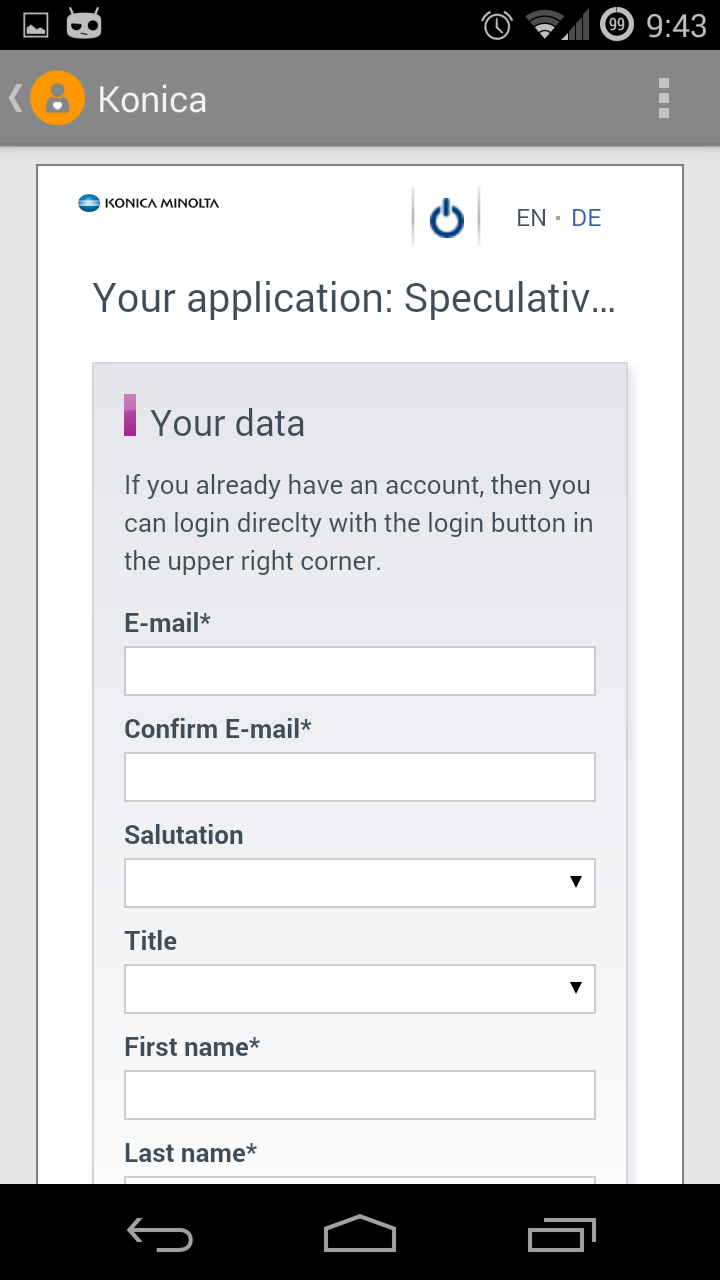
\includegraphics[width=.3\linewidth]{gfx/and/web}} \\
        \caption[Web View]{Web View}
\end{figure}

Let's go back to the navigation menu and click on search, or in Android's case, click the search icon in the top bar and type a search query. Once you start typing you'll notice the next difference. Android displays past searches as suggestions right underneath the search field. This feature was not implemented under iOS due to time constraints. Another big difference is that iOS can immediately begin to show results, while for Android to show the results, you need to click on 'Done'. This behavior is possible on Android, but requires a more complex implementation.

\begin{figure}[H]
        \myfloatalign
        \subfloat[iOS]
        {
\includegraphics[width=.3\linewidth]{gfx/ios/search}} \quad
        \subfloat[Android]
        {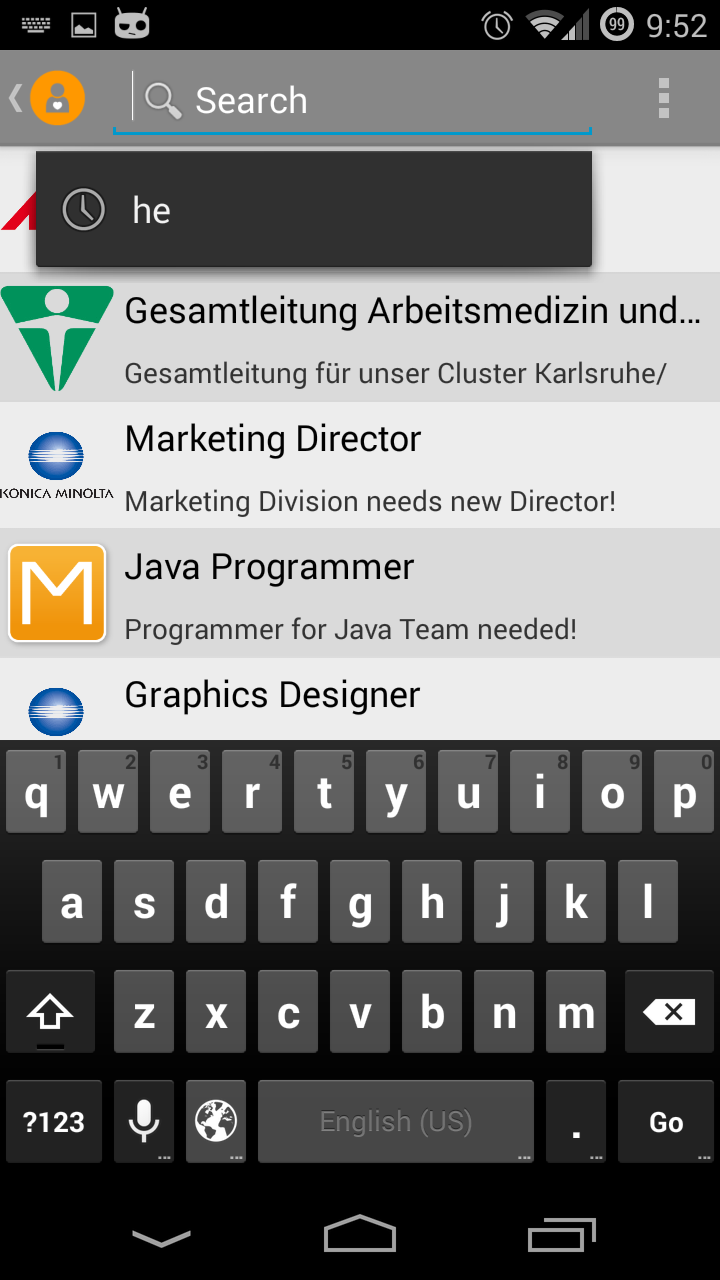
\includegraphics[width=.3\linewidth]{gfx/and/search}} \\
        \caption[Search View]{Search View}
\end{figure}

We can also refresh the main view, to see if new Publications have been made available. For this we need to go back to "Home" and, under iOS, pull the table down and release it, or, under Android, click on the refresh button.

\begin{figure}[H]
        \myfloatalign
        \subfloat[iOS]
        {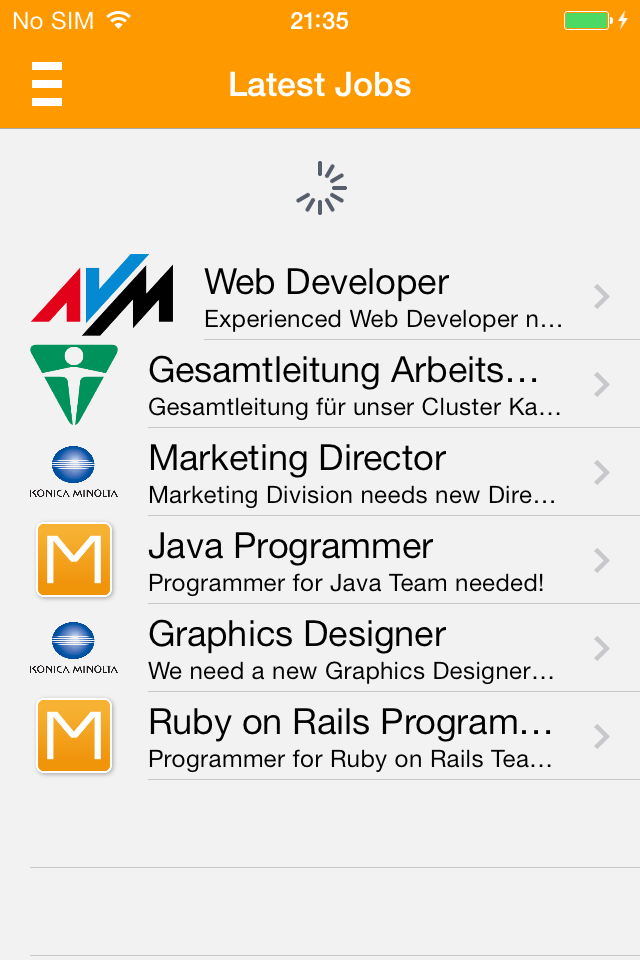
\includegraphics[width=.3\linewidth]{gfx/ios/refresh}} \quad
        \subfloat[Android]
        {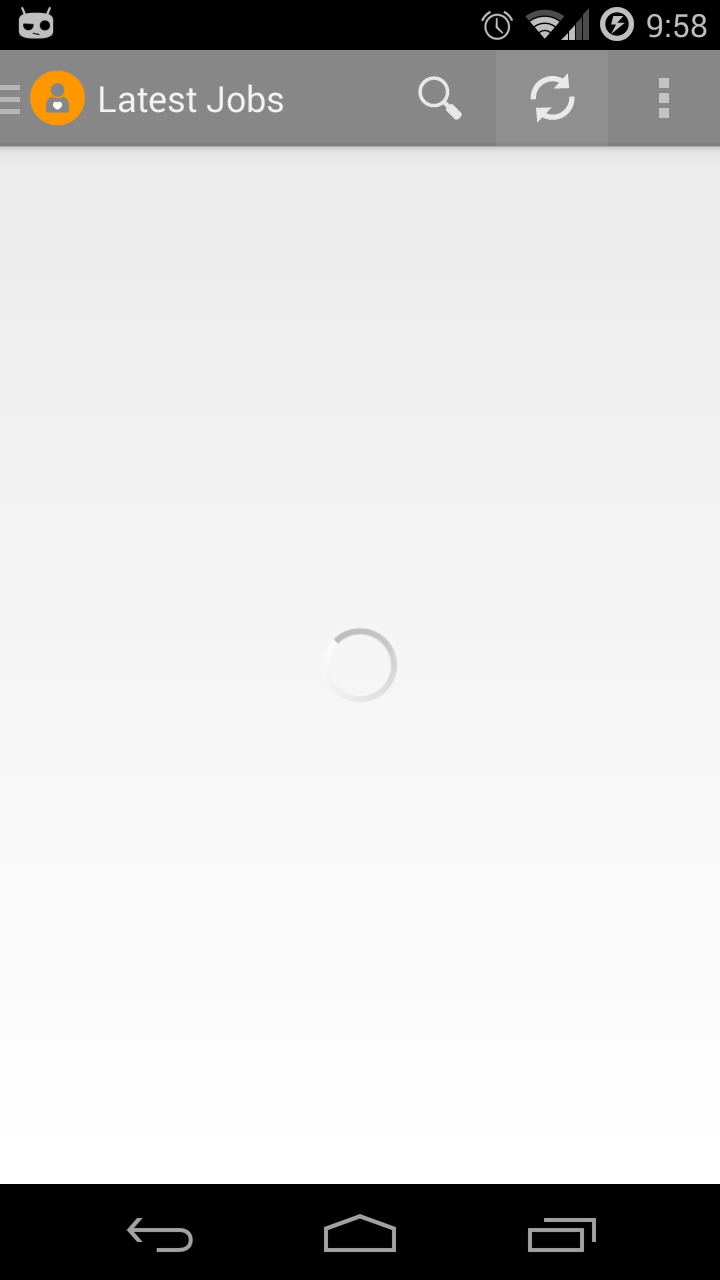
\includegraphics[width=.3\linewidth]{gfx/and/refresh}} \\
        \caption[Refreshing]{Refreshing}
\end{figure}
\newpage

There are also the possibility to display error messages, in case something goes wrong during the asynchronous connections.

\begin{figure}[H]
        \myfloatalign
        \subfloat[iOS]
        {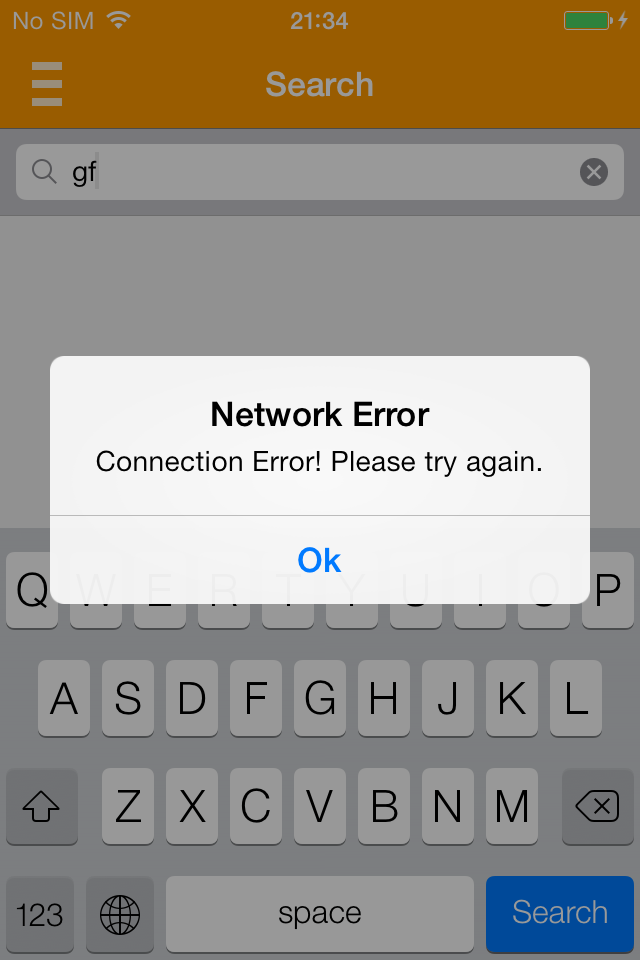
\includegraphics[width=.3\linewidth]{gfx/ios/error}} \quad
        \subfloat[Android]
        {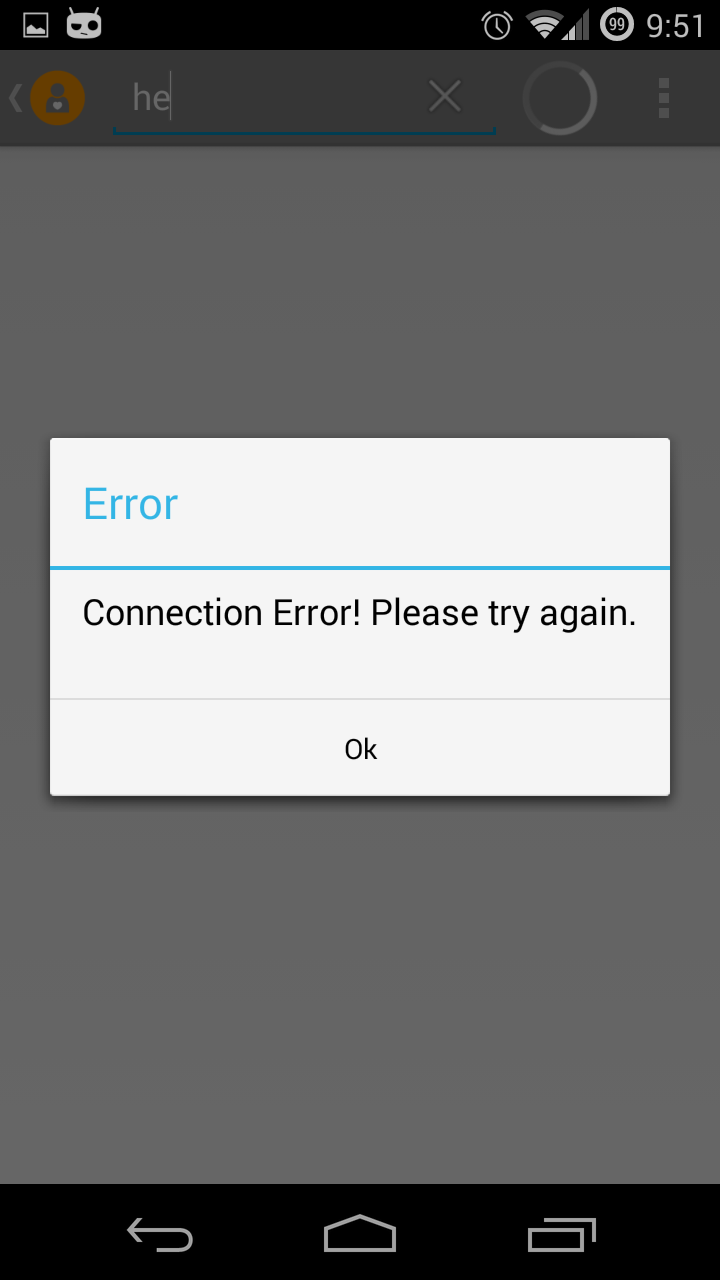
\includegraphics[width=.3\linewidth]{gfx/and/error}} \\
        \caption[Error Messages]{Error Messages}
\end{figure}

Another feature that should be displayed here is the ability to receive push notifications. Even though this functionality is implemented inside both applications, there is no server to actually send the notifications yet. This feature will be added to server soon and will be available once the application goes into production.





 

 